\documentclass[conference]{IEEEtran}
\IEEEoverridecommandlockouts

\usepackage{cite}
\usepackage{amsmath,amssymb,amsfonts}
\usepackage{algorithmic}
\usepackage{graphicx}
\usepackage{textcomp}
\usepackage{xcolor}
\def\BibTeX{{\rm B\kern-.05em{\sc i\kern-.025em b}\kern-.08em
    T\kern-.1667em\lower.7ex\hbox{E}\kern-.125emX}}
\begin{document}

\title{
Using Reinforcement Learning to Learn Novel Strategies
for Collective Decision Making \\
\thanks{
This research was sponsored by the U.S. Army Research Laboratory
and the U.K. Ministry of Defence
under Agreement Number W911NF-16-3-0001.
The views and conclusions contained in this document are those of the authors
and should not be interpreted as representing the official policies,
either expressed or implied, of the U.S. Army Research Laboratory,
the U.S. Government, the U.K.  Ministry of Defence or the U.K. Government.
The U.S. and U.K. Governments are authorized to reproduce and distribute
reprints for Government purposes notwithstanding any copyright notation hereon.
}
}

\author{
\IEEEauthorblockN{Hugo McNally, Sebastian Stein}
\IEEEauthorblockA{\textit{Electronics and Computer Science} \\
\textit{University of Southampton}\\
Southampton, UK\\
\{hm6g17, s.stein\}@soton.ac.uk}
\and
\IEEEauthorblockN{Malgorzata Turalska}
\IEEEauthorblockA{\textit{Network Science Division} \\
\textit{CCDC Army Research Laboratory}\\
Adelphi, MD, USA \\
mg.turalska@gmail.com}
\and
\IEEEauthorblockN{Rosie Lickorish, Geeth De Mel}
\IEEEauthorblockA{\textit{IBM Research Europe} \\
\textit{IBM}\\
Hursley, UK \\
\{rosie.lickorish, geeth.demel\}@uk.ibm.com}
}

\maketitle

\begin{abstract}
In military settings, collaborative decision making
is often used to solve large and complex problems under time pressure.
Here, workers can adopt
particularly promising solutions found by colleagues (imitation)
or independently explore new solutions (innovation).
However, there exists a trade-off between imitation and individual innovation
which has a consequential impact on the quality of the final solution found.
Therefore, the design of effective collaboration strategies
is an important problem when trying to find good solutions
to large and complex problems.
This paper formulates this strategy design as a reinforcement learning problem
and presents preliminary results
showing that, over short time periods, reinforcement learning outperforms
most handcrafted heuristics that are typically used in these settings.
\end{abstract}
\begin{IEEEkeywords}
collective decision making, NK-landscapes, collective intelligence,
problem solving, reinforcement learning
\end{IEEEkeywords}

\section{Introduction}\label{intro}
Collaborative decision making is utilised by most organisations,
including the military,
to find good solutions to large problems.
This is achieved due
to the large number of agents working on the problem simultaneously
and their ability to either
imitate promising solutions of their colleagues or neighbours,
or to innovate and discover better solutions independently.

The choices of agents to imitate as opposed to innovate,
can have a substantial impact on the time taken
for a good solution to be reached
and on the quality of the final solution found.
In addition to this,
the way in which an agent selects a neighbour to copy
also has a notable impact.

Two possible strategies that could be employed by an agent when deciding
which neighbour to copy are \emph{best member} and \emph{conformity}
\cite{sociallearning}.
The best member imitation strategy
copies the neighbour with the best solution,
if this solution is better than the agent's current solution.
The conformity imitation strategy, on the other hand,
will imitate one of the neighbours with the modal solution,
if their is a modal solution
and if this solution is better than the agent's own solution.
If an agent decides to only search when it fails to find a neighbour to imitate,
best member imitation will normally find a better solution than
conformity imitation in shorter time frames.
However, if the problem is complex,
best member imitation has a propensity to get stuck in local optima
due to the increased likelihood of imitation.
In comparison, conformity imitation gets closer to the global optimum
normally producing the better solution over a longer time frame.


This illustrates well the trade off between imitation and innovation,
with more imitation offering good solutions faster
but more inovation resulting in the better solution in the long run.
Reinforcement learning could offer valuable insights
into the best strategies to use for different problem complexities,
agent network topologies, and for given time budgets.
This paper preposes a way in which the collective learning scenarios
can be reframed as Finite Markov Decision Processes
and the preliminary results of a simple Q Learning approach,
before suggesting further experimentation
which could be carried out in this area.



\section{The Problem Space}

Following the literature, NK problem spaces will be used
as a proxy for problems faced by organisations of humans.
The N and K in their name are the two parameters
used to randomly generate them.
N is the number of binary traits or bits in the problem's solution space
and so a solution can be expressed as an integer in the range $(0, N]$.
K is the degree of epistasis equivalent to the complexity of the problem space,
as K increases from $0$ to $N-1$,
the ruggedness of the landscape increases and more local optima are introduced.
For this application,
the fitness or score of the solutions are normalised to values between 0 and 1,
before being passed through a monotonic function
which skews scores down.
This is done to reflect that the majority of randomly generated solutions,
are poor compared to the global optimum
in the real world problems faced by organisations \cite{monotonic}.

Individual innovation can be simulated by stepping through the solution space
by randomly flipping a bit of the solution.
A step is only taken if the resulting solution is better
than the solution previously held by the agent.


\section{Markov Decision Processes}\label{mdp}

A Markov Decision Process is a formalisation of decision making.
Unlike bandit problems which do not model situations where a decision
or `action' will effect the subsequent rewards,
a Markov Decision Process can model delayed rewards.
This is done by estimating the value function $q^{*}(s, a)$
which provides the estimated long term reward of action $a$ taken in state $s$,
as opposed to the stateless value function of bandit problems $q^{*}(a)$
\cite{RLbook2020}.

Reframing collective decision making as a Markov Decision Process
simply involves devising a way to express an agent's state
and provide actions which an agent is able to choose from.
Because the objective is to find a generalisable strategy
for problems of a given complexity,
the agent will learn over many different problems.
Therefore, the information and value
attributed to an agent's position on the landscape changes
and so is not valuable.
The time step the agent is in lends itself well to being a state.
For example, if the agents are greedy and all use best member imitation
at the beginning of a problem, they become clustered on similar solutions,
limiting their future reward.
However, at later time steps, best imitation could help bring stragglers
to more promising areas of the solution space.

Imposing a deadline (a number of time steps before an `episode' ends)
benefits the formulation
because it keeps the time space finite
and, in addition to this, it will allow one to explore
how the strategy learned by an agent changes with different time budgets,
an all too real constraint when solving real world problems.

%An alternative when the system does not improve for a few cycles stop.

Additional dimensions which could be added to an agent's state
are the agent's current score, its best performing neighbours' score,
the mean of all neighbours' scores
and the variance in all its neighbours' scores.
All of these could provide valuable situational awareness to the agent,
but the quantisation of these additional dimensions into discrete bins
requires careful consideration as elaborated upon in Section \ref{results}.

Two approaches can be taken when deciding upon
the actions available to an agent.
The simple approach is to have a number of preprogrammed strategies as actions,
for example the \emph{best member imitation else step}
and \emph{conformity imitation else step} strategies from the introduction.
An approach which will give the agent more freedom
and so may offer more insights into the optimal strategies,
is to split strategies into strategy components.
The strategies above would become an action set of
\emph{best member imitation}, \emph{conformity imitation} and \emph{step}.
When learning,
the agent would only be able to attempt a single action per time step
to learn the utility of each strategy component at each state.
When evaluated the agent can attempt the $n$ actions
with the highest perceived value in order of value,
essentially creating its own strategies.
This second approach will probably benefit more from Boltzmann distribution
off policy learning over a epsilon greedy policy,
because the actions are more likely to have more similar values.

There are also two approaches which can be taken when issuing rewards.
The agent's final score could be the only reward issued,
which would lend itself to Monte Carlo learning,
or the agent's improvement in score could be issued as a reward
at each time step,
which would lend itself to learning algorithms such as Q Learning.


\section{Preliminary Results}\label{results}

For the preliminary experiments,
the Q learning algorithm \cite{qlearning}
was used for its simplicity.
Initially a state space of the agent's current score
and the time step was used.
The agent's score was linearly quantised into 50 levels.
However, this state space resulted in poor performance,
which was likely due to quantisation.
With few solutions resulting in high scores due to the monotonic function,
high scores are rare.
A consequence of this is high score states being updated rarely,
reducing the agent's ability to learn the best actions to take at higher scores.
Because of this, the second set of simulations run used time step
as the only dimension of the state space.

\begin{figure}[htbp]
    \centering
    \centerline{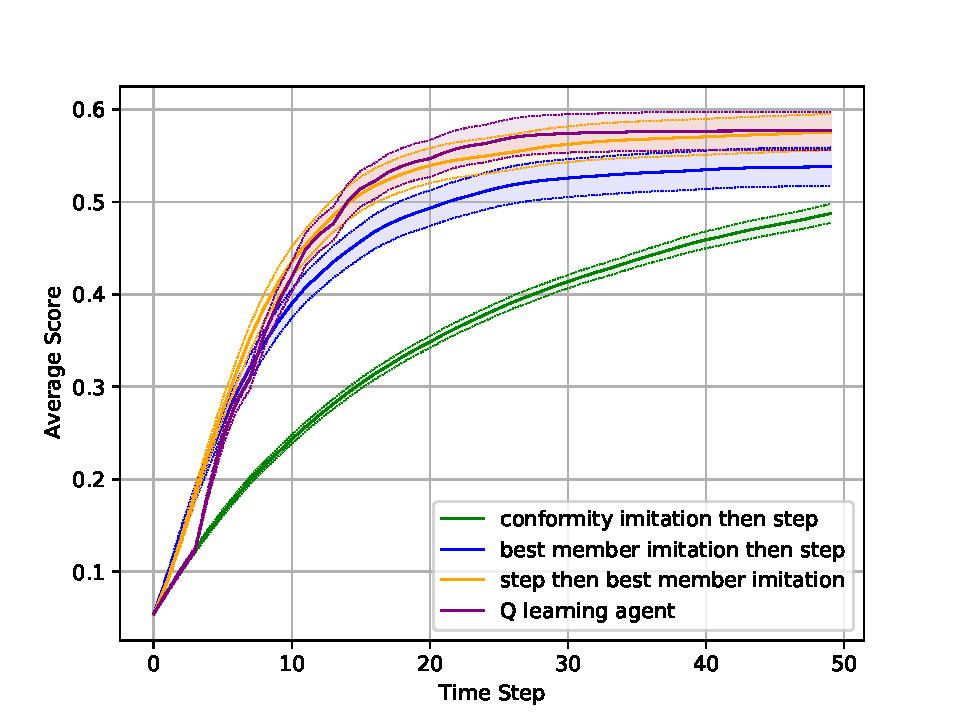
\includegraphics[scale=0.6]{figures/version4.pdf}}
    \caption{
        The average over 500 episodes of the agents' average score
        at each time step, with the 95\% confidence intervals
        plotted as dotted lines.
        Each episode a had a unique NK Landscape with N = 12 and K = 4
        and a regular network of agents with 60 vertices each with degree 4.
    }
    \label{avscore}
\end{figure}

The experiment shown in Figure \ref{avscore}
had a Q learning agent learn the value of three full strategy actions:
\emph{conformity imitation then step}, \emph{best member imitation then step},
or \emph{step then best member imitation}.
The Q learning agents were trained in a regular network with 60 vertices
each with degree 4, on random NK Landscapes with N = 12 and K = 4,
and with a deadline of 50 time steps.
The agent shown in Figure \ref{avscore}
used a epsilon greedy exploration with a epsilon decay from $1$ of $10^{-8}$,
had a learning rate of $0.6$ and a discount factor of $0.1$.
After training for 90100 episodes, around 7 hours of training,
can be seen to only perform marginally better
than the best of the original strategies after time step 14.

However, a promising trait of the Q learning agent's strategy is its
adherence to \emph{conformity imitation then step} in the first few time steps,
a strategy known to keep the number of unique solutions high.
This suggests the agent has learnt to avoid
agent clustering early in the simulation,
and seems to have enabled the agent to subsequently rise quickly
to the best solution at time step 15.
Its ability to hold this lead to the deadline
may improve with training time.




\section{Future Work}
Although the strategies produced by reinforcement learning are
not as capable as was hoped,
reinforcement learning does show promise
in its ability to identity good strategies for collective decision making.
Given more time experimenting with different
states spaces, actions spaces and learning techniques,
it is likely that reinforcement learning could offer valuable insights
into the best strategies to approach different problems with.

Environment noise will be a major factor in
the current Q Learning agent's sluggish learning.
This noise is due to the generation of a random NK landscapes for each episode,
each of which can favour very different strategies.
G Learning \cite{glearning}
could offer a solution to this problem.
It mitigates Q Learnings tendency to form a bias.
Not only this, but G Learning allows a prior to be used
which could be devised from heuristic techniques using existing research.

In addition to this,
some of the different formulations suggested in Section \ref{mdp}
could offer better insights into optimum strategies.
Chiefly among these would be the `strategy component' actions approach,
providing the agent with a lot more freedom.
Adding to this, only using a random subset of neighbours
has shown promising results \cite{sociallearning}
and would offer many more possible strategy components.
In a similar vein, different state spaces can be explored,
such as the agent's score with non-linear quantisation
which better reflects the frequency different scores.


Once reinforcement learning is performing well at high level strategy design,
one could have separate tables for different positions in the network.
For example, if the network has a hierarchical structure,
the agents at the higher `management' level could share a different table
to the agents at the lower `worker' level.
This would offer a valuable understanding of the difference in the
optimal decision making strategy between managers and workers.

This paper has focused on using reinforcement learning
to finding the best strategy
for a given network and complexity or range of networks and complexities.
There is also the alternative approach of using reinforcement learning to
find the optimal network structure for a given strategy.


\bibliography{refs}{}
\bibliographystyle{unsrt}

\end{document}
